\documentclass[conference]{IEEEtran}
\usepackage{amsmath,amssymb,graphicx,booktabs,url}
\usepackage{tikz}
\usetikzlibrary{arrows.meta,positioning}
\title{GNSS Re-entry after Outages: Admission Latency, Injected-Observation Exposure, and Position Error in a LIO Position Filter}
\author{\IEEEauthorblockN{Internal review draft: authors and affiliations unassigned}}
\begin{document}
\maketitle
\begin{abstract}
GNSS observations returning after an outage can be available before a position filter should use them. We study the tradeoff between the first actual GNSS update, exposure to injected biased observations, and position error in an outer position filter driven by FAST-LIO2 relative motion. A motion-validated recovery manager is compared with position-only fusion, innovation gating, Huber weighting, availability-based recovery, and a complete family of fixed qualification waits. The protocol separates measurement admission from offline error recovery, retains censored events, and reports every control even when it exceeds a service deadline. This initial manuscript registers the research question and analysis structure; new numerical results and any independent test are pending. Earlier R1 evidence does not establish improvement over long waits. This document is not submission ready.
\end{abstract}
\begin{IEEEkeywords}GNSS recovery, LiDAR--inertial odometry, admission latency, controlled stress evaluation\end{IEEEkeywords}
\section{Introduction}
The availability of a returned GNSS observation does not establish its reliability. Delaying its use can suppress injected bias, but also delays correction when the returned observations are useful. Position RMSE alone can reward a controller that simply waits until a finite artificial bias ends. A fair comparison therefore requires actual-update timing, exposure counts, and both short and extended position-error windows.

Our question is whether motion validation offers a useful empirical tradeoff under a stated re-entry service budget when compared with a full fixed-wait family. The R2 question was formulated after R1 results were known. Both building00 and parking00 have already been inspected and are seen data. An independent route, building01, can be evaluated only after source, configurations, inputs, and metrics are frozen. We do not claim universal optimality or novelty from a small benchmark.

\section{Related Work}
FAST-LIO2 supplies the LiDAR--inertial frontend~\cite{fastlio2}. KF-GINS is an independent GNSS/INS comparator~\cite{kfgins}. Innovation rejection and Huber weighting provide established robustness controls. The literature review will verify original GNSS-recovery and GNSS/LiDAR fusion mechanisms and distinguish them from the simpler outer position filter implemented here. No unimplemented published method will be presented as an executed baseline.

\section{System and Recovery Mechanism}
\begin{figure}[t]
\centering
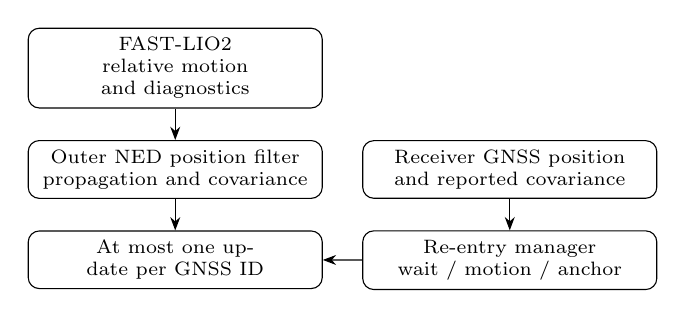
\begin{tikzpicture}[node distance=4mm, every node/.style={draw,rounded corners,font=\scriptsize,align=center,text width=35mm,minimum height=7mm},>=Stealth]
\node (lio) {FAST-LIO2\\relative motion and diagnostics};
\node[below=of lio] (prop) {Outer NED position filter\\propagation and covariance};
\node[right=5mm of prop] (gnss) {Receiver GNSS position\\and reported covariance};
\node[below=of gnss] (manage) {Re-entry manager\\wait / motion / anchor};
\node[below=of prop] (update) {At most one update per GNSS ID};
\draw[->] (lio)--(prop);\draw[->] (prop)--(update);\draw[->] (gnss)--(manage);\draw[->] (manage)--(update);
\end{tikzpicture}
\caption{Implemented framework. Reference trajectories and injection labels are used only for explicit initialization and offline evaluation.}
\end{figure}
The filter state is three-dimensional NED position. Relative motion is mapped into NED by a common initial orientation. With relative increment $\Delta\ell_k$, fixed alignment $A$, and process covariance $Q_k$,
\begin{equation}p_k^-=p_{k-1}^++A\Delta\ell_k,\qquad P_k^-=P_{k-1}^++Q_k.\end{equation}
The receiver reports an antenna position $z_k$ and component standard deviations. The innovation includes the antenna lever arm $b$:
\begin{equation}r_k=z_k-(p_k^-+R_{NB,k}b).\end{equation}
Receiver covariance is floored and, when admitted, inflated by robust weighting and the recovery policy. Each original GNSS ID can update the filter once. Relative GNSS differences serve as monitoring evidence rather than additional independent measurements. KF-GINS posterior positions are not injected into this filter.

The retained P-r03 manager combines an availability wait, GNSS-versus-LIO relative-motion consistency, and a past healthy anchor. It uses sensor diagnostics but no future reference or injection label. Its anchor can also veto a good observation when LIO drifts. Healthy-sensor fallback can admit a biased observation. The ablations remove motion checks, the anchor, or recovery decay. Exact equations and parameter provenance will be expanded from the frozen implementation before final review.

\section{Experimental Protocol}
\subsection{Data Roles and Common Foundation}
We reuse verified real-data caches and the existing deployment. All controls share the cache, initialization, process covariance, receiver-covariance floor, lever arm, clock mapping, and observed GNSS IDs. Cached backend timing is distinct from native frontend timing. The common initialization uses an explicitly declared reference condition; consequently these are initialization-conditioned errors, not a no-prior absolute geolocation experiment.

\subsection{Events and Measurement Clocks}
Primary contrasts are a 30-second observation deletion followed by unchanged observations and the same deletion followed by a 10-m artificial bias held for 90 seconds. The additional retained categories include short and clustered jumps, a 60-second deletion, a 3-m returned bias, and a ramp. Unchanged observations remain real receiver observations and need not be correct.
For the first actually present observation after deletion, let its measurement time be $t_{return}$. Let $t_{admit}$ be the first actual accepted KF update after that time. A state transition does not establish admission. Missing admission is right-censored at 180 seconds. We separately report conservative cache-availability timestamps because receiver arrival was not measured. Offline error recovery means position error below 3 m sustained for 5 s and is not a GNSS-admission metric.

\subsection{Complete Controls and Decision Rule}
The clock-only qualification durations are 2, 5, 10, 15, 30, 60, and 90 s on a common foundation. Qualification starts after the shared availability wait, so duration is not total admission latency. The primary service budget is 15 s; sensitivity budgets are 5, 10, 30, 60, and 90 s. Every wait remains in the full tables. Normal-interval cost is constrained by the best robust natural-case RMSE plus the larger of 2\% and 0.05 m. We report Pareto tradeoffs rather than optimizing a weighted latency/error score.

For every event, position error is evaluated on the same complete expected sample grid over 10, 30, 60, 90, and 180 s after return. Partial coverage and censored outcomes are retained. Exposure is the number and fraction of accepted artificially biased rows. It is a stress proxy, not a calibrated probability that a real GNSS observation is wrong.

\section{Results and Evidence Status}
\begin{table}[t]\centering\small
\caption{Registered evidence status at version r2\_r01.}
\begin{tabular}{lp{45mm}}\toprule
Item & Status\\\midrule
R1 identities & Raw files, caches, and frozen source verified\\
Full wait controls & Additional cache replay pending\\
R2 tradeoff metrics & Offline reanalysis pending\\
Independent building01 & Access audit pending; performance closed\\
Method increment & Not established\\
Publication novelty & Not established\\\bottomrule
\end{tabular}\end{table}
The R1 result and negative comparisons are retained. In particular, a long fixed wait can produce lower aggregate RMSE than the motion-validated manager under a finite injected bias. R2 will expose this comparison alongside its actual admission latency. All final numerical statements must map to a run, configuration hash, input hash, and an independently reproducible summary row. The final manuscript will include the full comparison table, latency/error tradeoff, a preordered representative recovery event, and ablations. Pending values are \texttt{TBD\_WITH\_EVIDENCE}; they are not estimates.

\section{Discussion and Limitations}
Seen-route analysis cannot validate generalization. The two building00 caches differ despite sharing inputs and a binary; this is a repeatability limitation and motivates paired cache sensitivity rather than treating them as independent samples. Artificial bias can cancel pre-existing receiver error; accepted injection counts therefore cannot alone identify field harm. Cached replay uses a declared availability bound and is not a measurement of live receiver arrival or end-to-end deployed latency. Event counts are small and correlated within each route. An unavailable independent route must be reported explicitly and cannot be replaced by relabeling parking00.

\section{Conclusion}
This version defines a transparent latency--exposure--error study and preserves the stronger long-wait comparison. The outcome, including a negative result, will determine the final empirical claims. It does not yet support a method increment or submission readiness.

\section*{Internal Review and AI Use}
This is an internal draft in a provisional IEEE conference layout. Official venue formatting, submission limits, disclosure wording, and author approval require verification. AI assistance was used for code orchestration, manuscript drafting, and evidence organization; human authors must verify all results and references. No authorship, funding, or formal submission is asserted.
\begin{thebibliography}{2}
\bibitem{fastlio2} W. Xu, Y. Cai, D. He, J. Lin, and F. Zhang, ``FAST-LIO2: Fast direct LiDAR-inertial odometry,'' \emph{IEEE Transactions on Robotics}, vol. 38, no. 4, pp. 2053--2073, 2022.
\bibitem{kfgins} i2Nav, ``KF-GINS: An EKF-based GNSS/INS integrated navigation system,'' source repository, \url{https://github.com/i2Nav-WHU/KF-GINS}.
\end{thebibliography}
\end{document}
